\section{PaTAS For Neural Networks}\label{sec:patas}

When parameters such as \( \theta_1 \) and \( \theta_2 \) are learned by backpropagation, their trustworthiness depends on the training data: mislabeled or biased samples compromise parameter trust. The SL opinion representation of \cref{sec:backsl} further distinguishes the causes of unreliability, with distrust arising from systematic issues such as mislabeled or poisoned data and uncertainty reflecting variability or noise in the assessment. A central challenge is how to exploit this distinction in practice.

\vspace{-0.5em}
\subsection{PaTAS General Description}

To address these challenges, we introduce the \emph{Parallel Trust Assessment System (PaTAS)}, which propagates trust assessments through a neural network by operating in parallel with the standard architecture and maintaining a structure mirroring its topology. It computes trust in the output from two sources: the trust in the input features at inference time, and the trust in the parameters, derived from the trustworthiness of the training dataset (covering both the features and the labels of the training samples). To extend the perceptron principles of the previous section, PaTAS associates a Trust Node with each neuron and connects the nodes according to the network's topology, forming a Trust Nodes Network (TNN).
\begin{definition}[Trust Nodes Network]
The \emph{Trust Nodes Network} is a structured composition of Trust Nodes, one per neuron of the underlying network, mirroring its architecture; it propagates trust across layers by applying trust-specific reasoning operations aligned with the neural computation flow.
\end{definition}

PaTAS continuously evaluates trustworthiness during inference: an input \(x\) may be trustworthy (high \(T_x\)) while the output \(y\prime\) is unreliable because of biased or poorly calibrated parameters \(\theta\) (low \(T_{y\prime}\)). Embedding trust operations inside the network would alter its computations, risk harming accuracy, and raise cost; PaTAS therefore performs trust assessment in parallel (Appendix~\ref{app:flow}), so that trust reasoning never interferes with the model's predictions.




\vspace{-0.5em}
\subsection{PaTAS Design}
\begin{figure}
    \centering
    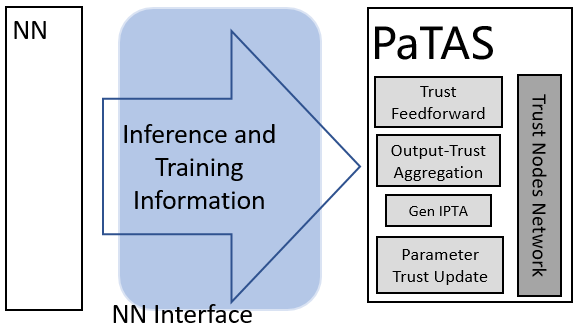
\includegraphics[width=0.43\linewidth]{good_figs/ptas/highPaTAS.png}
    \caption{High-Level Overview of PaTAS Integration with a Neural Network}
    \label{fig:highptas}
\end{figure}

% \subsection{PaTAS Components}\label{sec:ptasarch}



As illustrated in~\cref{fig:highptas}, PaTAS is composed of four main modules: Trust Feedforward, Output-Trust Aggregation, GenIPTA, and Parameter-Trust Update; the last parallels the role of backpropagation and receives a dedicated subsection.
\subsubsection{Trust Feedforward}

Trust Feedforward propagates trust through the Trust Node Network in alignment with the model's inference flow: at each layer, input and parameter trust are combined through the Trust Function's discounting and fusion. It produces a trust opinion per output neuron and stores the intermediate trust scores later used by the Parameter-Trust Update.

\subsubsection{Output-Trust Aggregation}

Output-Trust Aggregation combines the per-neuron output opinions into a single trust score via an SL fusion operator. Alternatively, one may read off the trust of the decided class directly: in digit classification, if the model predicts class `1', the decision trust is the opinion of that output Trust Node.

\subsubsection{Inference-Path Trust Assessment Generation(GenIPTA)}

GenIPTA dynamically constructs, for a single inference, an Inference-Path Trust Assessment (IPTA) reflecting the trustworthiness of the exact computational path taken: the activation trace recorded during that inference instantiates a temporary subnetwork containing only the Trust Nodes of the activated neurons. 

Since all neurons are typically activated to some degree while only a subset is strongly relevant, GenIPTA can also operate on truncated activation sets or weight the assessment by the activation values, so that stronger activations contribute more heavily. The functional flow of PaTAS across feedforward, backpropagation, and inference is illustrated in Appendix~\ref{app:flow}.

\vspace{-0.5em}
\subsection{Parameter-Trust Update}\label{sec:ptasfunc}
The Parameter-Trust Update adapts the trust of model parameters during training so that it reflects both the model's observed behavior and the reliability of the training data. To ground the design, recall the standard gradient-descent update for a parameter $\theta$:
\begin{equation}
\label{eq:gd1}
\theta \leftarrow \theta - l_r  \frac{\partial \mathcal{L}}{\partial \theta},
\end{equation}
where $l_r$ is the learning rate, $\mathcal{L}$ is the loss function, and $\frac{\partial \mathcal{L}}{\partial \theta}$ is the gradient. These gradients are computed recursively using the chain rule:
\begin{equation}
\label{eq:gd2}
\frac{\partial \mathcal{L}}{\partial \theta^{(l)}_{i,j}}
= \delta^{(l)}_i x^{(l-1)}_j,
\end{equation}
where $\theta^{(l)}_{i,j}$ denotes the weight connecting neuron $j$ in layer $(l-1)$ to neuron $i$ in layer $l$, $\delta^{(l)}_i$ is the error term of neuron $i$, and $x^{(l-1)}_j$ is the activation from the previous layer.

\Cref{eq:gd2} shows that gradients factor into an error term and an input activation, so parameter updates depend jointly on gradient signals, input activations, and learning dynamics; PaTAS mirrors this by using gradient information, input feature trust, and label trust as evidence in the Parameter-Trust Update. Notation is summarized in Appendix~\ref{app:symbols}; the complete procedure is \cref{alg:trustupdate}.

\begin{algorithm}
\caption{Parameter-Trust Update: revises each parameter's trust from gradient evidence, label trust, and neuron input trust under mini-batch training (helper functions in Appendix~\ref{app:algorithm}).}
\begin{algorithmic}[1]
    \Function{ParameterTrustUpdate}{$g, T_y, \epsilon$}
        \State $T_{y_\text{batch}}  \longleftarrow  \bigwedge_{y \in y_\text{batch}} T_y$ \Comment{aggregate label trust}
        \For{each layer $l$}
            \For{each neuron $n_i^{(l)}$}
                \State $g^{(l)}_i  \longleftarrow  \{\, g^{(l)}_{i,j} \;|\; j \in \mathcal{N}(i)\,\}$
                \State $T_{n_i \mid y_\text{batch}}  \longleftarrow $ \Call{NodeTrust}{$g^{(l)}_i, T_{y_\text{batch}}, \epsilon$}
                \State $T_{n_i \parallel Y_\text{batch}}  \longleftarrow $ \Call{DeduceTrust}{$T_{n_i \mid y_\text{batch}}, T_{n_i \mid \overline{y_\text{batch}}}, T_{y_\text{batch}}$}
                \For{each incoming edge $j$ to $n_i^{(l)}$}
                    \State $T_{\theta_{i,j}^{(l)}}  \longleftarrow $ \Call{Revise}{$T_{\theta_{i,j}^{(l)}}, T_{n_i \parallel Y_\text{batch}}$}
                    \State $T_{\theta_{i,j}^{(l)}} \longleftarrow $ \Call{Update}{$T_{\theta_{i,j}^{(l)}}, T_{x^{(l-1)}_j}, T_{y_\text{batch}}$}
                \EndFor
            \EndFor
        \EndFor
    \EndFunction
\end{algorithmic}
\label{alg:trustupdate}
\end{algorithm}
\Cref{alg:trustupdate} runs once per mini-batch over all layers and neurons. It first aggregates label trust, \(T_{y_\text{batch}} = \bigwedge_{y \in y_\text{batch}} T_y\), which conditions the trust in every parameter, then derives for each neuron \(n_i^{(l)}\) the opinion \( T_{n_{i}^{(l)} \mid y_\text{batch}} \) from gradient evidence, counting each incoming weight gradient with \( |g^{(l)}_{i,j}| < \epsilon\)\footnote{The threshold $\epsilon$ is not a tuned hyperparameter but a sensitivity parameter used only in \textsc{NodeTrust} to separate weak from strong gradients, selected relative to the typical gradient scale; it never affects model predictions or training dynamics.} as positive evidence \(r\) and the remainder as negative evidence \(s\), and mapping \((r,s)\) to a binomial opinion via \cref{eq:q1}. Since no evidence is available for the complementary case, \( T_{n_{i}^{(l)} \mid \overline{y_\text{batch}}} \) is vacuous, and the deduction operator \( \circledcirc \) combines the two conditionals with \( T_{y_\text{batch}} \) to give \( T_{n_{i}^{(l)} \parallel Y_\text{batch}} \).

For each incoming edge \(j\), the parameter trust is then revised with the deduced neuron trust, \(T_{\theta_{i,j}^{(l)}} \leftarrow T_{\theta_{i,j}^{(l)}} \circleddash T_{n_{i}^{(l)} \parallel Y_\text{batch}}\), and adjusted for the auxiliary factors that also drive the gradient update in \cref{eq:gd1,eq:gd2}, namely the learning rate, the input feature, and the batch labels:
\begin{equation}
    T_{\theta_{i,j}^{(l)}} \longleftarrow T_{\theta_{i,j}^{(l)}} \odot (T_{x_j^{(l-1)}} \oslash T_{y_\text{batch}}),
\end{equation}
where $\odot$ is binomial multiplication and $\oslash$ is the conservative combination \((b,d,u)\) with \(b = \min(b_1,b_2)\), \(d = \max(d_1,d_2)\), \(u = 1-(b+d)\). This reflects that both unreliable features and mislabeled data can strongly bias parameter updates: trust cannot exceed the weakest evidence and distrust must reflect the strongest warning. Bias terms receive the same treatment: each bias is handled as one additional parameter row whose input carries a vacuous opinion during propagation and whose trust opinion is revised exactly like any weight.

This process refines the trust in each parameter by incorporating both gradient-based behavioral evidence and auxiliary trust factors, allowing the PaTAS to align parameter trust with the training dynamics of the neural network. 

The mapping from gradient magnitude to evidence deserves explicit justification, since a large gradient does not, in isolation, imply an untrustworthy parameter. Two points make the interpretation well founded in PaTAS. First, evidence is \emph{relative}: gradients are not thresholded against an absolute constant but against the prevailing gradient scale through $\epsilon$, so the update reacts to a parameter that keeps receiving atypically large corrections \emph{after} the model has otherwise settled, not to the large gradients that are normal early in training. Second, evidence is \emph{conditional on label trust}: the same large gradient leads to a negative update of the trust assigned to the parameters only insofar as it is driven by data the model trusts. Under trusted labels, a parameter that the network must repeatedly and strongly correct is one whose learned value the trusted data does not support, which is precisely the signal PaTAS accumulates as reduced trust. Under distrusted or uncertain labels, the deduction through $T_{y_\text{batch}}$ discounts that same signal proportionally; the asymptotic cases are summarized in Appendix~\ref{app:asymptotic}. Gradient magnitude is nonetheless a proxy and can be confounded by learning-rate schedules, mini-batch noise, or saddle-point regions; a more direct evidence model for parameter reliability, together with an ablation over $\epsilon$ and gradient statistics, is left to future work.

\paragraph*{Computational Overhead}
PaTAS mirrors the network's computational flow over four-component opinions rather than scalars, so \(T_{\text{PaTAS}} \approx 3\,T_{\text{NN}}\) and \(T_{\text{with PaTAS}} \approx T_{\text{comm}} + 3\,T_{\text{NN}}\), with \(T_{\text{comm}}\) the communication overhead. Because training requires no value from PaTAS, the neural network can proceed while trust assessment completes.

\vspace{-0.5em}
\subsection{Theoretical Properties of PaTAS}\label{sec:ptastheory}
We first establish fundamental properties describing the stability and consistency of PaTAS.
\subsubsection{Convergence of PaTAS}
% \todo[inline]{Discuss convergence of PaTAS in case of convergence of input}
\label{sec:ptas_convergence}

During training, PaTAS revises the trust opinions on network parameters from trust opinions on the inputs, labels, hyperparameters, and gradient information, as outlined in \cref{alg:trustupdate}. Theorem~\ref{thm:convergence} establishes that this recursive update converges under an explicitly stated idealization of stable training; the training-time behavior under mini-batch noise is assessed empirically.

% Before delving into the specifics of PaTAS convergence, we first present a key theorem that will serve as a foundational tool in establishing the convergence properties of PaTAS.


\begin{theorem}[Convergence of PaTAS Creation]\label{thm:convergence}
\footnote{All proofs of the theorems in this section, as well as additional theoretical results, are provided in Appendix~\ref{app:proof}.}

Assume (i) the parameter opinions are initialized non-dogmatically (PaTAS initializes them as vacuous), and (ii) the per-batch revision opinion applied to each parameter stabilizes to a fixed opinion $q$: an idealization of a network trained to convergence with stationary gradient statistics and stable $T_x$, $T_y$, and $\epsilon$.
Let $T_\theta^{(n)}$ denote the trust opinion at iteration $n$ for parameter $\theta$. If the revision is performed as specified in \cref{alg:trustupdate}, then $T_\theta^{(n)}$ converges; for averaging-fusion revision the limit is $q$, at the geometric rate of Theorem~\ref{thm:arithm}.
\end{theorem}
Under actual mini-batch training the revision opinion fluctuates from batch to batch, so the theorem guarantees the consistency of the revision dynamics rather than convergence of the stochastic process itself; empirically, after accuracy convergence the trust trajectories oscillate within a narrow band around a stable level (Appendix~\ref{app:expres}).
\subsubsection{Symmetry and Invariance Properties of PaTAS}\label{sec:ptassyminv}

\begin{theorem}[Consistency Properties of PaTAS]\label{thm:infvac}
Let \(\omega^\emptyset=(0,0,1,a)\) be a vacuous binomial opinion and let \(\bar{x}=(d,b,u,a)\) denote the symmetric counterpart of \(x=(b,d,u,a)\). Then, for any parameter trust configuration \(T_\theta\):
\begin{enumerate}
    \item \emph{Vacuity is preserved.} Discounting a vacuous opinion is vacuous, \(\omega^A_B \otimes \omega^\emptyset = \omega^\emptyset\), and hence \(\mathrm{IPTA}(\omega^\emptyset) = \omega^\emptyset\).
    \item \emph{Inference is symmetric.} The outputs \(y = T_\theta(x)\) and \(\bar y = T_\theta(\bar x)\) satisfy \(u_y = u_{\bar y}\), \(b_y = d_{\bar y}\), and \(d_y = b_{\bar y}\). In particular a fully trusted input \((1,0,0)\) yields \(d_y = 0\), and a fully distrusted input \((0,1,0)\) yields \(b_{\bar y} = 0\).
\end{enumerate}
\end{theorem}

These properties are consistency guarantees rather than the paper's headline result: they establish that the trust computation is well behaved and justify reasoning about only the trusted-input case in the evaluation. Stronger, security-specific guarantees, such as provable bounds on trust degradation under a bounded poisoning adversary, are not claimed here and are left to future work.
